\documentclass[tikz,border=4pt]{standalone}
% Shared TikZ style for lecture figures
\usepackage{amsmath,amssymb}
\usepackage{tikz}
\usetikzlibrary{arrows.meta,calc,decorations.pathreplacing,patterns}
\definecolor{teal}{RGB}{38,150,140}
\definecolor{coral}{RGB}{230,95,75}
\definecolor{ink}{RGB}{20,45,60}
\tikzset{
  >={Stealth[length=2.6mm]},
  every picture/.style={line cap=round,line join=round,thick,ink},
  map/.style={->,thick},
  dot/.style={circle,fill,inner sep=1.2pt},
}

\begin{document}
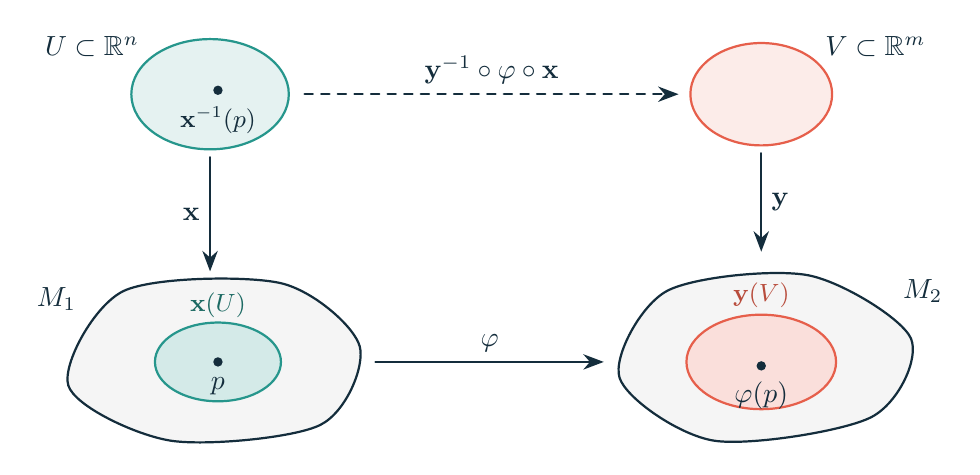
\begin{tikzpicture}
  % U in R^n
  \draw[fill=teal!12,draw=teal] (0,4) ellipse (1.0 and 0.7);
  \node[dot,label=below:{\small $\mathbf{x}^{-1}(p)$}] at (0.1,4.05) {};
  \node at (-1.5,4.6) {$U\subset\mathbb{R}^{n}$};
  % V in R^m
  \draw[fill=coral!12,draw=coral] (7,4) ellipse (0.9 and 0.65);
  \node at (8.45,4.6) {$V\subset\mathbb{R}^{m}$};
  % M_1
  \draw[fill=gray!8] plot[smooth cycle] coordinates {(-1.8,0.3) (-0.5,-0.4) (1.4,-0.2) (1.9,0.8) (0.9,1.6) (-1.1,1.5)};
  \node at (-1.95,1.4) {$M_{1}$};
  \draw[fill=teal!20,draw=teal] (0.1,0.6) ellipse (0.8 and 0.5);
  \node[teal!70!black] at (0.1,1.32) {\small $\mathbf{x}(U)$};
  \node[dot,label=below:{$p$}] at (0.1,0.6) {};
  % M_2
  \draw[fill=gray!8] plot[smooth cycle] coordinates {(5.2,0.4) (6.4,-0.4) (8.4,-0.1) (8.9,0.9) (7.6,1.7) (5.8,1.5)};
  \node at (9.05,1.5) {$M_{2}$};
  \draw[fill=coral!20,draw=coral] (7.0,0.6) ellipse (0.95 and 0.6);
  \node[coral!80!black] at (7.0,1.45) {\small $\mathbf{y}(V)$};
  \node[dot,label=below:{$\varphi(p)$}] at (7.0,0.55) {};
  % maps
  \draw[map] (0,3.2) -- node[left] {$\mathbf{x}$} (0,1.75);
  \draw[map] (7,3.25) -- node[right] {$\mathbf{y}$} (7,2.0);
  \draw[map] (2.1,0.6) -- node[above] {$\varphi$} (5.0,0.6);
  \draw[map,dashed] (1.2,4.0) -- node[above] {$\mathbf{y}^{-1}\circ\varphi\circ\mathbf{x}$} (5.95,4.0);
\end{tikzpicture}
\end{document}
